\documentclass[11pt]{article}
% anderweitig wiederverwendbare Makros fuer Diss
\usepackage{amsfonts}

% allgemeine mathematische Notation
\newcommand{\ceil}[1]{\left\lceil #1\right\rceil}
\newcommand{\floor}[1]{\left\lfloor #1\right\rfloor}
\newcommand{\abs}[1]{\left| #1\right|}
\newcommand{\seq}[1]{\langle #1\rangle}
\newcommand{\norm}[1]{\left\|#1\right\|}
\newcommand{\enorm}[1]{\norm{#1}_{2}}
\newcommand{\sumnorm}[1]{\norm{#1}_{1}}
\newcommand{\maxnorm}[1]{\norm{#1}_{\infty}}
\newcommand{\xor}{\oplus}
\newcommand{\set}[1]{\left\{ #1\right\}}
\newcommand{\gilt}{:}
\newcommand{\sodass}{\,:\,}
\newcommand{\setGilt}[2]{\left\{ #1\sodass #2\right\}}
\newcommand{\Def}{:=}
\newcommand{\zvektor}[2]{\left(#1,#2\right)}
\newcommand{\vektor}[2]{\left(\begin{smallmatrix}#1\\#2\end{smallmatrix}\right)}
\newcommand{\condition}[1]{\left[#1\right]}
\newcommand{\binomial}[2]{\binom{#1}{#2}}
\newcommand{\even}{\mathrm{even}}
\newcommand{\odd}{\mathrm{odd}}
\newcommand{\mymod}{\,\bmod\,}
\newcommand{\divides}{|}

\newcommand{\blank}{\Box}
\newcommand{\cross}[2]{\langle #1,#2 \rangle}
\newcommand{\defeq}{\mathrel{:=}}
\newcommand{\hash}{\sym{@}}
\newcommand{\hD}[1][D]{^{(#1)}}
\newcommand{\hed}[1][D]{^{1/#1}}
\newcommand{\Lpal}{L_{\mathrm{pal}}}
\newcommand{\Lparity}{L_{\mathrm{parity}}}
\newcommand{\Lvv}{L_{\mathrm{vv}}}
\newcommand{\pD}[1][D]{^{[#1]}}
\newcommand{\pos}[1]{\mathbf{#1}}
\newcommand{\qs}{\mathord{\Box}}
\newcommand{\mSet}[2]{\left\{#1 \mid #2\right\}}
\newcommand{\s}{\mathord{-}}
\newcommand{\CAce}{\hbox{\mdseries\scshape CAce}}
\newcommand{\sCAce}{\s\CAce}
\newcommand{\CAcs}{\hbox{\mdseries\scshape CAcs}}
\newcommand{\sCAcs}{\s\CAcs}
\newcommand{\CAww}{\hbox{\mdseries\scshape CAww}}
\newcommand{\sCAww}{\s\CAww}
\newcommand{\sC}{\s\hbox{\scshape Chng}}
\newcommand{\sD}{\s\hbox{\scshape Diam}}
\newcommand{\sT}{\s\hbox{\scshape Time}}
\newcommand{\CA}{\hbox{\mdseries\scshape CA}}
\newcommand{\sCA}{\s\CA}
\newcommand{\ST}[1]{\langle #1\rangle}
\newcommand{\sym}[1]{\mathord{\hbox{\texttt{\upshape #1}}}}

% Typen
\newcommand{\nat}{\mathbb{N}}
\newcommand{\natnull}{\mathbb{N}_{0}}
%\newcommand{\natless}[1]{\mathbb{N}_{<#1}}
\newcommand{\natless}[1]{\mathbb{N}_{#1}}
\newcommand{\nplus}{\mathbb{N}_+}
\newcommand{\real}{\mathbb{R}}
\newcommand{\rplus}{\mathbb{R}_+}
\newcommand{\rnneg}{\mathbb{R}_*}
\newcommand{\integer}{\mathbb{Z}}
% \newcommand{\intint}[2]{\set{#1,\ldots, #2}}
\newcommand{\intint}[2]{{#1}..{#2}}
\newcommand{\realrange}[2]{\left[#1, #2\right]}
\newcommand{\realrangeo}[2]{\left(#1, #2\right)}
\newcommand{\realrangelo}[2]{\left(#1, #2\right]}
\newcommand{\realrangero}[2]{\left[#1, #2\right)}
\newcommand{\unitrange}[2]{\realrange{0}{1}}
\newcommand{\bool}{\set{0,1}}
%\newcommand{\boolean}{\mathbb{B}}
%\newcommand{\mapping}[2]{#1\rightarrow #2}
\newcommand{\mapping}[2]{{#2}^{#1}}
\newcommand{\powerset}[1]{{\cal P}\left(#1\right)}
\newcommand{\NP}{\mathbf{NP}}
\newcommand{\Bild}{\mathbf{Bild}\:}

% Typannotation
\newcommand{\withtype}[1]{\in#1}

% Wahrscheinlichkeitsrechnung
\newcommand{\prob}[1]{{\mathbf{P}}\left[#1\right]}
\newcommand{\condprob}[2]{{\mathbf{P}}\left[#1\;|\;#2\right]}
\newcommand{\condexpect}[2]{{\mathbf{E}}\left[#1\;|\;#2\right]}
\newcommand{\expect}{{\mathbf{E}}}
\newcommand{\var}{{\mathbf{Var}}}
\newcommand{\quant}[2]{\tilde{#1}_{#2}}

% asymptotische Notation
\newcommand{\whpO}[1]{\tilde{\mathrm{O}}\left( #1\right)}
\newcommand{\Oschlange}{$\tilde{\mathrm{O}}$}
\newcommand{\Ohh}[1]{\mathcal{O}\!\left( #1\right)}
\newcommand{\Oh}[1]{\mathcal{O}\!\left( #1\right)}
\newcommand{\oh}[1]{\mathrm{o}\!\left( #1\right)}
\newcommand{\Th}[1]{\Theta\!\left( #1\right)}
\newcommand{\Thsmall}[1]{\Theta( #1)}
\newcommand{\Om}[1]{\Omega\!\left( #1\right)}
\newcommand{\om}[1]{\omega\!\left( #1\right)}
\newcommand{\Oleq}{\preceq}

% local reference
\newcommand{\lref}[1]{\ref{\labelprefix:#1}}
\newcommand{\llabel}[1]{\label{\labelprefix:#1}}
\newcommand{\labelprefix}{} % later redefined using renewcommand

% Diskussion
\newcommand{\discussionsize}{\small}
\newenvironment{discussion}{\par\discussionsize}{\par}

% open issues
%\marginparwidth5cm
\marginparpush2mm
%\newcommand{\frage}[1]{\makebox[0cm]{$\bigotimes$}\marginpar{\tiny #1}}
%\newcommand{\frage}[1]{{\sf[ #1]}\marginpar{?}}
\newcommand{\frage}[1]{}

\newcommand{\mysubsubsection}[1]{\vspace{2mm}\noindent{\bf #1 }}

% punkt am ende von display math
\newcommand{\punkt}{\enspace .}

% Pseudocode Unterst\"utzung
\newenvironment{code}{\noindent%\sf%
\begin{tabbing}%
\hspace{2em}\=\hspace{2em}\=\hspace{2em}\=\hspace{2em}\=\hspace{2em}\=%
\hspace{2em}\=\hspace{2em}\=\hspace{2em}\=\hspace{2em}\=\hspace{2em}\=%
\kill}{\end{tabbing}}

% 1=pos, 2=llable, 3=caption
\newcommand{\labelcommand}{}
\newcommand{\captiontext}{}
\newsavebox{\codeparam}
\newcounter{lineNumber}
\newenvironment{disscodepos}[3]{%
\renewcommand{\labelcommand}{#2}%
\renewcommand{\captiontext}{#3}%
\sbox{\codeparam}{\parbox{\textwidth}{#3}}%
\begin{figure}[#1]\begin{center}\begin{code}\setcounter{lineNumber}{1}}{%
\end{code}\end{center}\caption{\llabel{\labelcommand}\captiontext}\end{figure}}

\newenvironment{disscode}[2]{\begin{disscodepos}{htb}{#1}{#2}}%
{\end{disscodepos}}

% code in text 
%\newcommand{\codel}[1]{{\sf #1}}
%\newcommand{\codem}[1]{\mathsf{#1}}
\newcommand{\codel}[1]{\mbox{\rm "`#1"'}}
\newcommand{\codem}[1]{\mathrm{#1}}

\newcommand{\id}{\tt}
\newcommand{\Function} {{\bf Function\ }}
\newcommand{\Procedure}{{\bf Procedure\ }}
\newcommand{\Process}{{\bf process\ }}
\newcommand{\While}    {{\bf while\ }}
\newcommand{\Repeat}   {{\bf repeat\ }}
\newcommand{\Until}    {{\bf until\ }}
\newcommand{\Loop}     {{\bf loop\ }}
\newcommand{\Exit}     {{\bf exit\ }}
\newcommand{\Goto}     {{\bf goto\ }}
\newcommand{\Do}       {{\bf do\ }}
\newcommand{\Od}       {{\bf od\ }}
\newcommand{\Dopar}       {{\bf dopar\ }}
\newcommand{\For}      {{\bf for\ }}
\newcommand{\Step}      {{\bf step\ }}
\newcommand{\Foreach}      {{\bf foreach\ }}
\newcommand{\Rof}      {{\bf rof\ }}
\newcommand{\Forall}      {{\bf forall\ }}
\newcommand{\To}       {{\bf to\ }}
\newcommand{\If}       {{\bf if\ }}
\newcommand{\Is}       {:=}
\newcommand{\Endif}    {{\bf endif\ }}
\newcommand{\Fi}       {{\bf fi\ }}
\newcommand{\Then}     {{\bf then\ }}
\newcommand{\Else}     {{\bf else\ }}
\newcommand{\Elsif}    {{\bf elsif\ }}
\newcommand{\Return}   {{\bf return\ }}
\newcommand{\Set}      {{\bf set\ }}
\newcommand{\Boolean}  {{\bf boolean\ }}
\newcommand{\Integer}  {$\integer$}
\newcommand{\True}     {{\bf true\ }}
\newcommand{\False}    {{\bf false\ }}
\newcommand{\Bitand}   {{\bf bitand\ }}
\newcommand{\Var}      {{\bf var\ }}
\newcommand{\Xor}       {{\bf\ xor\ }}
\newcommand{\Not}       {{\bf\ not\ }}
\newcommand{\Or}       {{\bf\ or\ }}
\newcommand{\Div}       {{\bf\ div\ }}
\newcommand{\Mod}       {{\bf\ mod\ }}
\newcommand{\End}       {{\bf end\ }}
\newcommand{\Endfor}       {{\bf endfor\ }}
\newcommand{\Rem}[1]   {{\bf (*~}{\rm#1}{\bf ~*)}}
% rechtsbuendiger Kommentar
%\newcommand{\RRem}[1]   {\`{$\mathbf{(*}$~ }{\rm#1}{~$\mathbf{*)}$}}
\newcommand{\RRem}[1]   {\`{\bf --\hspace{0.5mm}--~}{\rm#1}}
\newcommand{\RRemNL}[1]   {\`{\bf (*~ }{\rm#1}{\bf ~*)}%
{\tiny\arabic{lineNumber}}\stepcounter{lineNumber}}

\newcommand{\At}[1]{\left\langle#1\right\rangle}
\newcommand{\NL}{\`{\tiny\arabic{lineNumber}}\stepcounter{lineNumber}}

% Parallelverarbeitungspseudocode
\newcommand{\iProc}{i_\mathrm{PE}}

% Parameter 1=pos, 2=xsize, 3=filename, 4=llabel, 4=caption
\newcommand{\dissepslong}[5]{\begin{figure}[#1]\begin{center}%
\epsfxsize#2\leavevmode\epsfbox{#3.eps}%
\end{center}\caption{\llabel{#4}#5}\end{figure}}

\newcommand{\dissepspos}[4]{\dissepslong{#1}{#2}{\labelprefix/#3}{#3}{#4}}
\newcommand{\disseps}[3]{\dissepspos{htb}{#1}{#2}{#3}}

% Beweise
\newdimen\endofsize\endofsize=0.5em
\def\endofbeweis{~\quad\hglue\hsize minus\hsize
                 \hbox{\vrule height \endofsize width
\endofsize}\par}
% gibt es in amsmath schon
\newenvironment{myproof}{\begin{proof}}{\endofbeweis\end{proof}}
% \newcommand{\platsch}{\hglue\hsize minus\hsize}



\usepackage[utf8]{inputenc}
%\usepackage{algorithmic}
\usepackage{placeins}
\usepackage{tabularx}
%\usepackage{algorithm}
\usepackage{amssymb,amsmath,amsthm}
\usepackage{color}
\usepackage{fullpage}     
\usepackage{latexsym}
\usepackage{makeidx}
\usepackage{multicol}
\usepackage{numprint}
\usepackage{t1enc}
\usepackage{times}
\usepackage{graphicx}
\usepackage{url}
\usepackage[left=2cm,top=1.5cm,right=2cm]{geometry}

\usepackage[]{algorithm2e}
\usepackage[noend]{algpseudocode}
\npdecimalsign{.} % we want . not , in numbers

\definecolor{mygrey}{gray}{0.75}
\newcommand{\ie}{i.e.\ }
\newcommand{\etal}{et~al.\ }
\newcommand{\eg}{e.g.\ }
\newcommand{\Id}[1]{\ensuremath{\text{{\sf #1}}}}

\def\MdR{\ensuremath{\mathbb{R}}}
\def\MdN{\ensuremath{\mathbb{N}}}
\newcommand{\mytodo}[1]{{\color{blue}#1}}
\newcommand{\sout}[1]{{\color{mygrey}#1}}

\newcommand{\mytitle}{ {\color{red}KaLP} v1.00 -- {\color{red}Ka}rlsruhe {\color{red}L}ongest {\color{red}P}aths \\ User Guide}
\begin{document}
\title{\mytitle}
\author{Tomas Balyo, Kai Fieger and Christian Schulz\\ 
	\textit{Karlsruhe Institute of Technology (KIT)},
	\textit{Karlsruhe, Germany} \\
	\textit{Email: \{\url{balyo}, \url{christian.schulz}\}\url{@kit.edu}}, \url{fieger@ira.uka.de} }
\date{}

\maketitle
\begin{abstract}
This paper severs as a user guide to the longest paths framework KaLP (Karlsruhe Longest Paths). We give a rough overview of the techniques used within the framework and describe the user interface as well as the file formats used. 
\end{abstract}

\tableofcontents
\thispagestyle{empty}

\vfill
\pagebreak
\section{Introduction}
The longest path problem (LP) is to find a simple path 
of maximum length between two given vertices of a graph 
where length is defined as the number of edges or the total weight of the edges in the path.
The problem is known to be NP-complete~\cite{NP} and has several applications such as designing circuit boards~\cite{Circuit1,Circuit2}, project planning~\cite{Brucker}, information retrieval~\cite{Wong} or patrolling algorithms for multiple robots in graphs~\cite{Multirobot}. 
For example, when designing circuit boards where the length difference between wires has to be 
kept small~\cite{Circuit1,Circuit2}, the longest path problem manifests itself when the length of shorter wires is supposed to be increased. 
Another example application is project planning/scheduling where the problem can be used to determine the least 
amount of time that a project could be completed in~\cite{Brucker}. 

The purpose of the manual is to give a very rough overview over the techniques used in the programs, as well as to serve as a guide and manual on how to use our algorithms. 
We start with a short overview of the algorithms implemented within our framework. 
This is followed by a description of the graph format that is used. 
It is basically the same graph format that is used by Metis~\cite{karypis1998fast} and Chaco~\cite{chaco}, as well as the DIMACS graph format. We then give an overview over the user interface of KaLP.
\vfill
\pagebreak

\section{Longest Paths by Dynamic Programming}
We now give a rough overview over the algorithms implemented in our framework. For details on the algorithms and further improvements, we refer the interested reader to the corresponding papers. 
Our algorithm solves the longest path problem (LP) for weighted undirected graphs. We restrict ourselves here to introducing the main approach.
%TODO which includes preprocessing the graph as well as combining paths. 

\subsection{Exhaustive Depth First Search}
\label{sec:approach}
A simple way to solve the longest path problem is \emph{exhaustive depth-first search}~\cite{stern}. 
In regular depth-first search (DFS) a vertex has two states: marked and unmarked. Initially, all vertices are unmarked. The search starts by calling the DFS procedure with a given vertex as a parameter. This
vertex is called the root.
The current vertex (the parameter of the current DFS call) is marked and then the DFS procedure is recursively executed on each unmarked vertex reachable by an edge from the current vertex. The current vertex is called the parent of these vertices. Once the recursive DFS calls are finished we backtrack to the parent vertex. The search is finished once DFS backtracks from the root vertex.
\begin{figure}[b]
\begin{algorithm}[H]
% \KwData{this text}
% \KwResult{how to write algorithm with \LaTeX2e }
\SetKwProg{Fn}{Search}{}{}
\Fn{exhDFS($v$)}{
\If{$v$ is unmarked}{
   mark $v$\;
   \ForEach{$ \{v,w\} \in E$}{
   	exhDFS($w$)\;
   }
   unmark $v$\;
  }
}
\end{algorithm}
 \caption{Exhaustive depth first search. In order to solve LP we start this search from the start vertex and update the best found solution each time the (unmarked) target vertex is found.}
\label{exDFS}
\end{figure}

Exhaustive DFS is a DFS that unmarks a vertex upon backtracking. Pseudocode can be seen in Figure \ref{exDFS}. In that way every simple path 
in the graph starting from the root vertex is explored. The LP problem can be solved with 
exhaustive DFS by using the start vertex as the root. During the search the 
length of the current path is stored and compared to the previous best 
solution each time the target vertex is reached. If the current length is greater than 
that of the best solution, it is updated accordingly. When the search is done 
a path with maximum length from $s$ to $t$ has been found. If we store the length of the longest path for each vertex (not just the target vertex), then all the longest simple paths from $s$ to every other vertex can be computed simultaneously.

\subsection{Algorithm Overview}
\label{sec:algorithm_overview}
\begin{figure}
\centering
\begin{tabular}{cc}
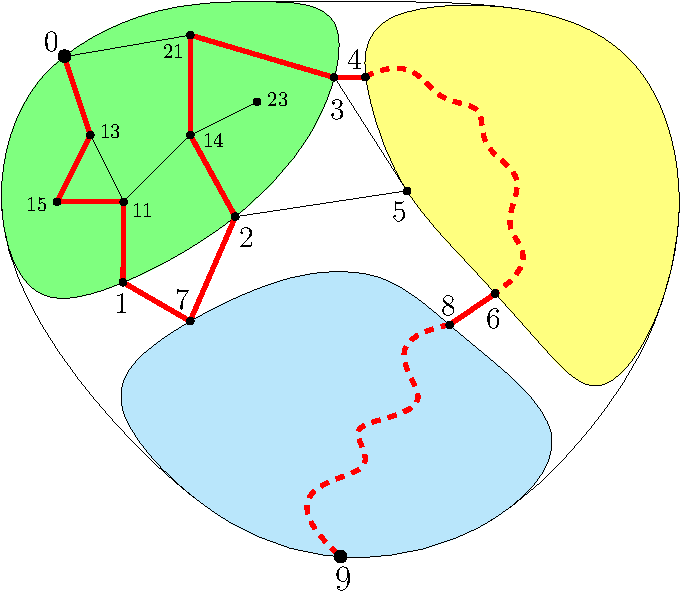
\includegraphics[scale=0.75]{examplegraph}&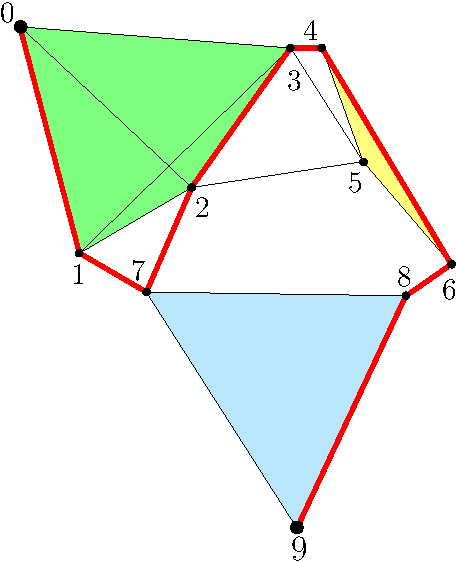
\includegraphics[scale=0.75]{exampleauxiliary}
\end{tabular}
\caption{On the left we see an example graph $G = (V, E)$. We want to calculate the longest path between $s = 0$ and $t = 9$. The initial block $B=V$ is partitioned into three subblocks $B_{green},  B_{yellow}$ and $B_{blue}$. The vertices $0,1,\ldots, 9$ are the boundary vertices of these subblocks. The edges between the subblocks are boundary edges. The right graph is the auxiliary graph that is constructed by the LPDP algorithm. A search path of LPDP can be seen on the right. Its induced boundary vertex pairs for the subblocks are: $P_{green} = \{\{0,1\}, \{2,3\}\}$, $P_{yellow} = \{\{4,6\}\}$, $P_{blue} = \{\{7,7\}, \{8,9\}\}$. The corresponding candidate for the longest path is shown on the left in red.
}
\label{fig:lpdpexample}
\end{figure}
Dynamic programming requires us to be able to divide LP into subproblems. In order to do this we first generalize the problem\\

\noindent\fbox{%
    \parbox{\textwidth}{%
       \underline{Given:} A graph $G=(V,E)$, $s,t \in V$, $B \subseteq V$ and $P \subseteq \{\{a,b\} \mid a,b \in b(B) \}$\\
       where $b(B) := \{ v \in B \mid v = s \lor  v = t \lor \exists{} \{v,w\} \in E : w \notin B \}$ are the $boundary$ $vertices$ of $B$.\\
\\
\underline{Problem:} Find a simple path from $a$ to $b$ in the subgraph induced by $B$ for every $\{a,b\} \in P$.\\
Find these paths in such a way that they do not intersect and have the maximum possible cumulative weight. 
    }%
}
\\

We explain an example of the problem with Figure \ref{fig:lpdpexample}. Later this figure will be used to explain the LPDP algorithm further, but for now we only look at the green area on the left. This green area represents a subgraph of a graph G. This subgraph is induced by the set $B = \{0, 1, 2, 3, 11, 13, 14, 15, 21, 23\}$. The vertices 0 and 9 in the figure are the vertices s and t of the problem's definition. This results in the boundary vertices $b(B) = \{0, 1, 2, 3\}$. If we restrict the figure to the green subgraph, there are two paths shown in red. These paths represent a solution to the problem if $P = \{\{0,1\},\{2,3\}\}$. This solution has a weight of 7 as the graph is unweighted and the two paths consist of 7 edges.\\


We make the following observations about the problem:
\newtheorem{observation}{Observation}
\begin{observation}[The structure of $P$]\label{structureOfP}
The set $P$ of a solvable problem can contain pairs of the form $\{v,v\}$. The problem is impossible to solve if $P$ contains two pairs $\{a,b\}$ and $\{b,c\}$.
\end{observation}
\begin{proof}
A pair $\{v,v\} \in P$ results in a path of weight 0 that consists of a single vertex ($v$) and no edges. Two pairs $\{a,b\},\{b,c\} \in P$ would result in two intersecting paths as they would have the same start- or end-vertex $b$.
\end{proof}

\begin{observation}\label{unsolvable}
If the problem is unsolvable for a $P$, it is also unsolvable for any $P' \supseteq P$. 
\end{observation}
%\begin{proof}
%\end{proof}
 \noindent The proof is trivial.

\begin{observation}[Subproblems]\label{subproblem}
A solution of the problem for $B$ and $P$ also induces a solution to the problem for any $B' \subseteq B$ and a $P'$: Restricting the solution to vertices of $B'$ results in non-intersecting, simple paths in the subgraph of $B'$. These paths start and end in boundary vertices of $B'$ inducing the set $P'$. These paths are the solution to the problem for $B'$ and $P'$.
\end{observation}
\begin{proof}
Otherwise we could take the solution for $B$ and $P$, remove all paths in the subgraph of $B'$ and replace them with the solution for $B'$ and $P'$. We would obtain a solution for $B$ and $P$ with a higher cumulative weight than before. This is impossible.
\end{proof}

LP is a special case of this problem where $B = V$  and $P = \{\{s,t\}\}$. Observation \ref{subproblem} is the basis of the LPDP algorithm as it allows us to recursively divide LP into subproblems. 
LPDP requires a hierarchical partitioning of the graph. Level 0 represents the finest level of partitioning. On each higher level we combine a group of blocks from the lower level into a single larger block. On the highest level we are left with a single block $B = V$. We solve our problem for each of these blocks and any possible $P$: We start by calculating the solutions for each block of level 0. We then calculate the solutions for a block on level 1 by combining the solutions of its level 0 subblocks. This is repeated level by level until we calculated all solutions for the block $B = V$, namely the solutions for $P= \{\{s,t\}\}, \{\}, \{\{s,s\}\}, \{\{t,t\}\}$ and $\{\{s,s\}, \{t,t\}\}$. The latter four are trivial (see observation \ref{structureOfP}) and do not have to be calculated. With solution for $P= \{\{s,t\}\}$ we also solved LP as it is the longest path from $s$ to $t$.

The next section shows how we calculate the solutions for one block $B$ with the help of its subblocks from the level below. The initial solutions for the blocks on level 0 can be calculated with the same algorithm. In order to do this we interpret each vertex $v$ as a separate subblock. We know the solutions for each of these subblocks ($P= \{\}$ or $\{\{v,v\}\}$). So we can use the same algorithm to calculate solutions for the blocks on level 0.

\subsection{Combining Solutions}
\label{sec:combsolutions}
Let $P_S$ be the set of boundary vertex pairs for a set of vertices $S$. Given is a subset of vertices $B \subseteq V$ and a partition $B_1$,\ldots,$B_k$ of $B$ ($B_1\cup\cdots\cup B_k=B$ and $B_i\cap B_j=\emptyset$ for $i\neq j$). We assume that we already solved the problem for each $B_i$ and every possible $P_{B_i}$. We calculate the solution for $B$ and every possible $P_B$ with the following algorithm:

We construct an auxiliary graph $G' = (V', E')$ with $V' = \bigcup\limits_{i=1}^{k} b(B_{i})$. $E'$ contains all edges $\{v,w\} \in E$ where $v \in b(B_i)$ and $w \in b(B_j)$ (with $i \neq j$). We call these edges boundary edges. They keep the weight they had in $G$. We also create a clique out of the boundary vertices of every $B_i$. These new edges have a weight of 0. An example of this can be seen in Figure \ref{fig:lpdpexample}. The graph on the left is partitioned into three blocks $B_{green},  B_{yellow}$ and $B_{blue}$. On the right we can see the constructed auxiliary graph. For now we can ignore the path that is shown in red.

In order to calculate the solutions for $B$ we start a modified version of the exhaustive DFS on every boundary vertex of $B$. Pseudocode of this search algorithm is called LPDP-Search and is shown in Figure \ref{lpdpsearch}. Compared to exhDFS LPDP-Search works with multiple paths. This way the search algorithm resembles a nested exhDFS. The first path starts from a starting boundary vertex $b_1$. Once another boundary vertex $b_2$ of $B$ is reached, LPDP-Search has two options. It can traverse the graph's edges as usual, but it also is able to jump to other unused boundary vertices. If LPDP-Search jumps to another boundary vertex $b_3$, we completed a path from $b_1$ to $b_2$ and a new path from $b_3$ is started. This induces the pair $\{b_1,b_2\} \in P_B$. At any point of the search $P_B$ is equivalent to the boundary vertex pairs induced by the completed paths. The sets $P_{B_i}$ are maintained the following way: The paths contain an edge $\{v,w\}$ of the $B_i$-clique $\iff \{v,w\} \in P_{B_i}$. If the paths contain a vertex $v \in B_i$ but no edge $\{v,w\}$ of the $B_i$-clique: $\{v,v\} \in P_{B_i}$. During the search we do not traverse an edge that would induce a $P_{B_i}$ without a solution. Further traversal of a path with an unsolvable $P_{B_i}$ only leads to $P'_{B_i} \supseteq P_{B_i}$ which is still unsolvable (as already mentioned in observation \ref{unsolvable}).

\begin{observation}[Alternative representation of $P$]\label{MX}
We can transform~$P$ into two sets $(M,X)$: $\{x,y\} \in P \land x \neq y \iff \{x,y\} \in M$ and $\{x,x\} \in P \iff x \in X$. We imagine a clique consisting of the boundary vertices $b(B)$. This way we can interpret $M$ as a set of edges in this clique. It follows from observation \ref{structureOfP} that $M$ represents a matching (set of edges without common vertices) in that clique.
\end{observation}

Each time we complete a path we calculated a candidate for the solution to $B$ and $P_B$. The weight of this candidate is the weight of the solution of each block $B_i$ and the induced $P_{B_i}$ plus the weight of all boundary edges in the paths. Until now no $P_B$ found by the search contains a pair $\{v,v\}$ as we do not allow a path to end in its starting boundary vertex. This way $P_B$ is equivalent to a $M$ and $X = \emptyset$ according to the representation in the observation \ref{MX}. So when we complete a path we additionally go through all possible sets $X$ (while modifying the sets $P_{B_i}$ accordingly) and update the best found solution for these candidates as well.

An example can be seen in Figure \ref{fig:lpdpexample}. In the auxiliary graph on the right we traversed a path from 0 to 9. We found a solution for $P = \{\{0,9\}\}$. The induced boundary vertex pairs for the subblocks are $P_{green} = \{\{0,1\}, \{2,3\}\}$, $P_{yellow} = \{\{4,6\}\}$, $P_{blue} = \{\{7,7\}, \{8,9\}\}$. When we look up these solutions for the subblocks we obtain the path that is shown on the left.

An important optimization which can be seen in Figure \ref{lpdpsearch} in line \ref{lpdp:vga} is that we only allow a path to end in a boundary vertex with a higher ID than its starting boundary vertex. Additionally, a path can only start from a boundary vertex with a higher ID than the starting vertex of the previous path (line \ref{lpdp:startpaths}). The first optimization essentially sorts the two vertices of each pair $\{x,y\} \in P$. The second then sorts these pairs. Resulting in an order and a direction in which we have to search each path in $P$. This avoids unnecessary symmetrical traversal of the graph.

\begin{figure}
\LinesNumbered
\begin{algorithm}[H]
\SetKwProg{Fn}{Search}{}{}
\Fn{LPDP-Search($v$)}{
% \everypar={\nl}
\If{$v$ is unmarked $\&$ $\forall i :$ there exists a solution for $B_i$ and  $P_{B_i}$}{ \label{lpdp:marked}
   mark $v$\;
   \If{$v \in b(B)$}{
	\If{already started some $\{a,.\}$-path}{
		\If{$v > a$}{\label{lpdp:vga}
			$P_B \gets P_B \cup \{\{a,v\}\}$ \tcp*{completes the $\{a,v\}$-path} \label{lpdp:endpath}
			update\_solutions()  \label{lpdp:updatesolutions}\;
			\ForEach{$w \in b(B)$ where $w > a$}{ \label{lpdp:startpaths}
   				LPDP-Search($w$) \tcp*{starts a $\{w,.\}$-path} \label{lpdp:firstcall}
   			}
   			$P_B \gets P_B \setminus \{\{a,v\}\}$ \tcp*{resume search with $\{a,.\}$-path} \label{lpdp:resume}
		}
   	}%{
   	%	start a $\{v,.\}$-path\;
   	%}
   }
   \ForEach{$ \{v,w\} \in E$}{ \label{lpdp:traverse}
   	LPDP-Search($w$)\; \label{lpdp:secondcall}
   }
   unmark $v$\;
}
}
\end{algorithm}
 \caption{Basic search algorithm that LPDP uses to search the auxiliary graphs.}
\label{lpdpsearch}
\end{figure}


\subsection{Parallelization}
\label{sec:parallel}
\begin{figure}[]
  \centerline{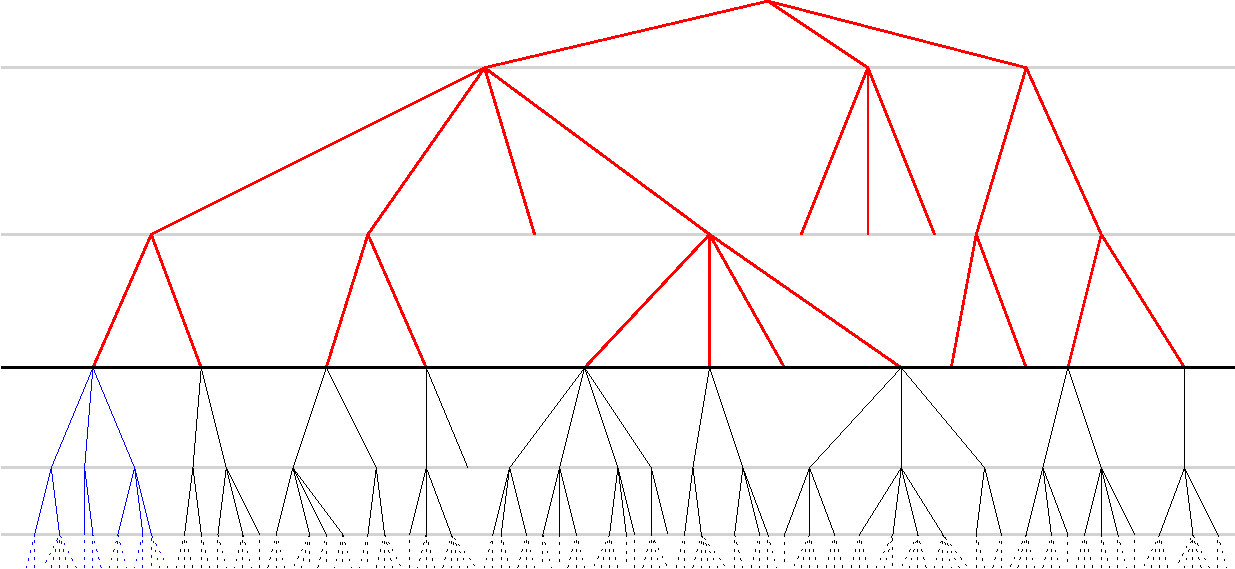
\includegraphics[width=\linewidth]{split}}
 \caption{Recursion tree of LPDP-Search}
  \label{fig:recursiontree}
 \end{figure}

In order parallelize LPDP we use an approach that is inspired by the ``Cube and Conquer'' approach for SAT-Solving that was presented by Heule et al. \cite{heule}. In this paper a SAT formula is partitioned into many subformulas. These subformulas can be solved in parallel. We can do something similar for LPDP by partitioning the search space of LPDP-Search into many disjunct branches. We do this by running LPDP-Search from each boundary vertex with a limited recursion depth. Every time the search reaches a certain level of recursion the search stores its current context in a list and returns to the previous recursion level. Figure \ref{fig:recursiontree} shows an example of this. We can see a LPDP-Search limited to 3 recursions in red. A stored context represents all the data that allows us to continue the search at this point later on. The created list of contexts is then used as a queue. Each element of the queue represents a branch of the search that still has to be executed. One such branch can be seen in blue in Figure \ref{fig:recursiontree}. We execute these branches in parallel. Each time a thread finishes one branch it receives the next branch from the top of the queue. This automatically results in a form of load balancing.

\FloatBarrier
\pagebreak
\section{Graph Format}
\label{ss:graphformat}
\subsection{Input File Format}
We use two file formats: the Metis/Chaco format and the DIMACS graph format. 

\paragraph*{Metis/Chaco Graph Format.}The first graph format used by our programs is the same as used by Metis \cite{karypis1998fast}, Chaco \cite{chaco} and the graph format that has been used during the 10th DIMACS Implementation Challenge on Graph Clustering and Partitioning. If you want to use this format, your filename has to end with the ``.graph'' extension.
The input graph has to be undirected, withoud self-loops and without parallel edges.

To give a description of the graph format, we follow the description of the Metis 4.0 user guide very closely. A graph $G=(V,E)$ with $n$ vertices and $m$ edges is stored in a plain text file that contains $n+1$ lines (excluding comment lines). The first line contains information about the size and the type of the graph, while the remaining $n$ lines contain information for each vertex of $G$. Any line that starts with \% is a comment line and is skipped.

The first line in the file contains either two integers, $n$ $m$, or three integers, $n$ $m$ $f$. The first two integers are the number of vertices $n$ and the number of undirected edges of the graph, respectively. Note that in determining the number of edges $m$, an edge between any pair of vertices $v$ and $u$ is counted \emph{only once} and not twice, \ie we do not count the edge $(v,u)$ from $(u,v)$ separately. The third integer $f$ is used to specify whether or not the graph has weights associated with its vertices, its edges or both. If the graph is unweighted then this parameter can be omitted. It should be set to $1$ if the graph has edge weights, 10 if the graph has node weights and 11 if the graph has edge and node weights.

The remaining $n$ lines of the file store information about the actual structure of the graph. In particular, the $i$th line (again excluding comment lines) contains information about the $i$th vertex. Depending on the value of $f$, the information stored in each line is somewhat different. In the most general form (when $f=11$, \ie we have node and edge weights) each line has the following structure:
\begin{center}
       $c\, v_1\, w_1\, v_2\, w_2 \ldots v_k\, w_k$ 
\end{center}
where $c$ is the vertex weight associated with this vertex, $v_1, \ldots, v_k$ are the vertices adjacent to this vertex, and $w_1, \ldots, w_k$ are the weights of the edges. Note that the vertices are numbered starting from 1 (not from 0). Furthermore, the vertex-weights and edge-weights must be integers greater or equal to 0. However, note that vertex-weights are ignored by our algorithm. 
\begin{figure}[h!]
\begin{center}
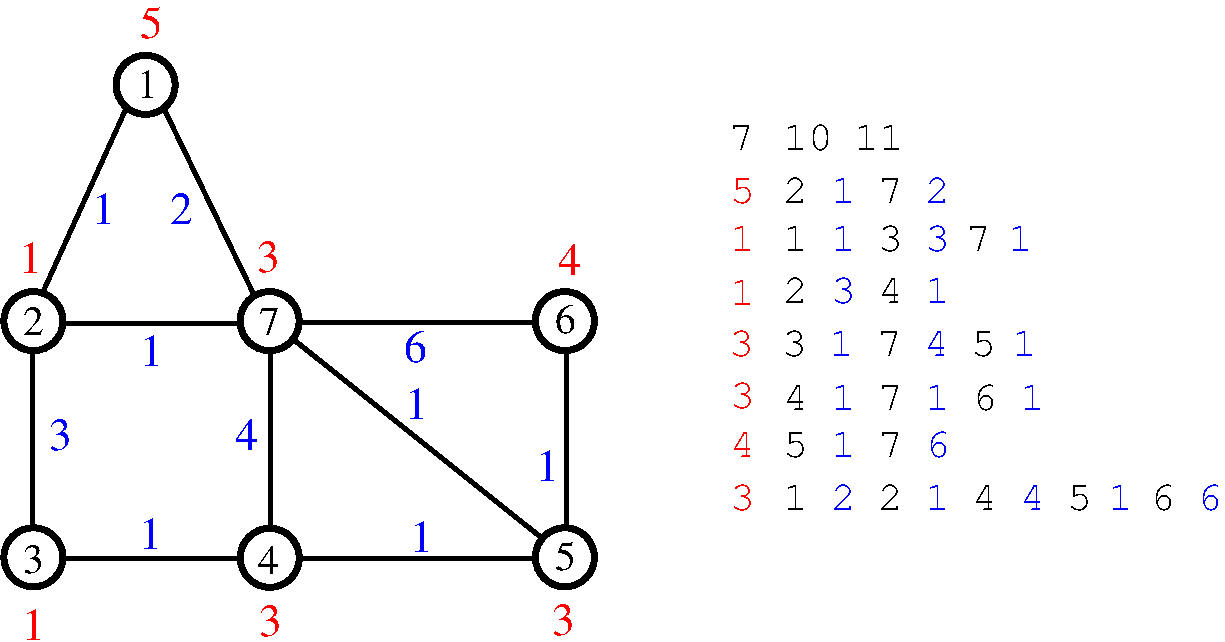
\includegraphics[width=.6\textwidth]{example_graph.pdf}
\end{center}

\caption{An example graph and its representation in the Metis/Chaco graph format. The IDs of the vertices are drawn within the cycle, the vertex weight is shown next to the circle ({\color{red}red}) and the edge weight is plotted next to the edge ({\color{blue}blue}).}
\label{fig:example}
\end{figure}

\paragraph*{DIMACS Graph Format.}
The second graph format that our software can read is the DIMACS graph format from the 9th DIMACS Implementation challenge. 
Here, a graph contains $n$ nodes and $m$ arcs. Nodes are identified by integers $1\ldots n$. 
Graphs in the format can be interpreted as directed or undirected, depending on the problem being studied. However, for our software to work correctly, there needs to be a backward edge for each directed edge, \ie the graph needs to be undirected.
Arc weights are signed integers.
By convention, graph file names should have the suffix ``.gr'' or ``.dimacs''. 
Line types are as follows: 
\begin{itemize}
        \item comment lines can appear anywhere and are ignored by programs. Example: ``c This is a comment''.
        \item the problem line is unique and must appear as the first non-comment line. Example ``p sp n m''. Here, $n$ is the number of nodes and $m$ is the number of arcs.
        \item arc descriptor lines describe arcs and their weights. Example: ``a u v w''. Here, $u$ is the source vertex, $t$ is the target vertex and $w$ is the weight/length associated with the arc.
\end{itemize}
An example file for the graph from Figure~\ref{fig:example}: \\

\noindent
\textit{
        p sp 10 22 \\
        c this is a comment \\
        c the graph contains 10 nodes and 22 arcs \\
        c node ids are numberd in 1..10 \\
        a 1 2 1 \\
        a 1 7 2\\
        a 2 1 1\\
        a 2 3 3\\
        a 2 7 1\\
        a 3 2 3\\
        a 3 4 1\\
        a 4 3 1 \\
        a 4 7 4 \\
        a 4 5 1\\
        ....
}
\vfill
\pagebreak
\subsection{Output File Formats}
\subsubsection{Path File}
We now specify our output format. 
This file contains $\ell+1$ lines where $\ell$ is the number of edges in the longest path.
Let $p := v_1, v_2, \ldots, v_{\ell}$ be the longest path from $s=v_1$ to $t=v_\ell$.
In each line the ID of the corresponding vertex is given, \ie line $i$ contains the ID of the vertex $v_i$ (here the vertices are numbered from 0 to $n-1$).
\subsection{Troubleshooting}
KaLP should not crash! If KaLP crashes it is mostly due to the following reasons: the provided graph contains self-loops or parallel edges, there exists a forward edge but the backward edge is missing or the forward and backward edges have different weights, or the number of vertices or edges specified does not match the number of vertices or edges provided in the file.
In case of the METIS format, please use the \emph{graphchecker} tool provided in our package to verify whether your graph has the right input format. If our graphchecker tool tells you that the graph that you provided has the correct format and KaLP crashes anyway, please write us an email.

\vfill
\pagebreak
\section{User Interface}
KaLP contains the following programs: kalp, graphchecker, generate\_maze. To compile these programs you need to have Argtable, Threading Building Blocks (TBB), g++ and scons installed (we use argtable-2.10, g++-4.8.0 and scons-1.2). Once you have that you can execute \emph{compile.sh} in the main folder of the release. When the process is finished the binaries can be found in the folder \emph{deploy}. We now explain the parameters of each of the programs briefly.
\subsection{KaLP}
\paragraph*{Description:} This is the longest path program. 
\paragraph*{Usage:\\} 

steps threads

\begin{tabular}{ll}
kalp &   file  -{}-start\_vertex=<int> -{}-target\_vertex=<int> [-{}-threads=<int>] [-{}-steps=<int>] [-{}-help]\\
       &  [-{}-print\_path] [-{}-partition\_configration=<string>] [-{}-output\_filename=<string>] \\
\end{tabular}
                          
\subsection*{Options:\\}

\begin{tabularx}{\textwidth}{lX}
  file                        & Path to graph file that you want to partition. \\
  -{}-help                      & Print help. \\
  -{}-start\_vertex=<int> & Start vertex to use. \\
  -{}-target\_vertex=<int> & Target vertex to use. \\
  -{}-threads=<int> & Number of threads to use. Default: 1 for serial execution\\
  -{}-steps=<int> & Number of steps used to divide the workload for parallel execution. Equivalent to the recursion depth limit that was explained in section \ref{sec:parallel}\\
  -{}-print\_path & Printing the solution at the end of the program.  \\
  -{}-partition\_configuration=<string> & Use a configuration for the partitioning tool. (Default: eco) [strong|eco|fast]. We recommend to use the strong configuration on difficult instances. \\
  -{}-output\_filename=<string>               & Output filename. If specified the vertices of the longest path will be written into that file. \\
\end{tabularx}
%\vfill
%\pagebreak
\subsection{Generate Maze}
\paragraph*{Description:} This is a program that generates a maze, from that generates a graph and writes the graph to disc using the DIMACS format..
\paragraph*{Usage:\\} 
\begin{tabular}{ll}
generate\_maze & [-{}-help] [-{}-output\_filename=<string>] [-{}-seed=<int>] \\
               &  [-{}-width=<int>] [-{}-height=<int>] [-{}-blocked=<double>] [-{}-print\_path]
\end{tabular}


\subsection*{Options:\\} 
\begin{tabularx}{\textwidth}{lX}

  -{}-help                        &           Print help. \\
  -{}-output\_filename=<string>    &           Filename of the outputfile. Default: grid.dimacs \\
  -{}-seed=<int>                    &         Seed to use for random number generator. \\
  -{}-width=<int>                    &        Width of the maze. Default: 10 \\
  -{}-height=<int>                    &       Height of the maze. Default: 10 \\
  -{}-blocked=<double>                 &      Percentage of cells in the maze to be blocked. Default: 0.3 (i.e. 30\%) \\
  -{}-print\_path                       &      Printing the solution at the end of the program. \\

\end{tabularx}

\subsection{Graph Format Checker}
\paragraph*{Description:} This program checks if the graph specified in a given file is valid (only for METIS file format). 
\paragraph*{Usage:\\} 
\begin{tabular}{ll}
graphchecker & file
\end{tabular}
\subsection*{Options:\\} 
\begin{tabularx}{\textwidth}{lX}
  file                       & Path to the graph file. \\
\end{tabularx}

\vfill
\pagebreak
\bibliographystyle{plain}
\bibliography{citations,phdthesiscs}
\end{document}


